\documentclass[a4paper,11pt,openany]{book} % bez prazdnych stran
%\documentclass[a4paper,11pt]{book} % s prazdnymi stranami, aby kapitola zacinala na neparnej, vhodne pre tlac

% definovanie kompilatora (magic comment):
% !TeX program = xelatex

% ============== PREAMBULA ==============
% (nacitanie balikov a podobne)
% ============== PREAMBULA ==============
% (nacitanie balikov a podobne)
% Ctrl+klik na balik zobrazi dokumentaciu k baliku (v TeXstudiu)
% Je tu vela uzitocnych balikov ak ale nejaky nepotrebujete, zakomentujte ho

%definovanie verzie dokumentu (pdf/tlacena)
\usepackage{etoolbox}
\newbool{printVersion} % premenna pre volbu verzie
%\booltrue{printVersion} % tlacena: odkomentovat, pdf: nechat zakomentovanie


% geometria a formatovanie stran
\pagestyle{plain} % defaultny styl stran (plain/headings/empty/myheadings)
\ifbool{printVersion}{
	\usepackage[top=2.5cm, bottom=2.5cm, left=3.5cm, right=2cm]{geometry} % odporucane okraje
}{
	\usepackage[top=2.5cm, bottom=2.5cm, left=2.75cm, right=2.75cm]{geometry} % okraje vhodnejsie do pdf (rovnaka sirka vlavo/vpravo) 
}

% jazyk
\usepackage[main=slovak,english]{babel}  % primarny jazyk: SK, dalsie jazyky: EN


% bibliografia
\usepackage[style=iso-numeric,backend=bibtex,giveninits=true,sorting=nyt]{biblatex}
\addbibresource{literatura.bib}


% fromatovanie
\usepackage{indentfirst} % odsadenie prveho odstavca
\usepackage{enumitem} % číslovanie ((a),(b),(c),... i), ii), iii),...)
\usepackage[small]{caption} % male popisy obrazkov


% grafika
\usepackage{graphicx} % obrazky
\usepackage{subcaption} % podobrazky (subfigure)
\graphicspath{ {./figures/} } % priecinok s obrazkami
\usepackage{wrapfig} % obrazky obtekane textom
\usepackage[dvipsnames]{xcolor} % farby (dvipsnames pridava dalsie farby)
\usepackage{colortbl} % farebne tabulky
\usepackage{multirow} % treba pre merge-ovanie budniek v tabulkach

\usepackage{pdfpages} % vlozenie stran z ineho pdf (musi byt za graphics)


% matematika
\usepackage{mathtools} % rozsirenie zakladneho matematickeho balika amsmath
\usepackage{amssymb} % dalsie symboly a fonty (napriklad pre mnozinu realnych cisel)
\usepackage[locale=DE]{siunitx} % jednotky SI

% Definície, Vety, Dôkazy...
\usepackage{amsthm}
\theoremstyle{definition}
\newtheorem{thm}{Veta}[chapter]
\newtheorem{defn}[thm]{Definícia}
\newtheorem{lem}[thm]{Lemma}
\newtheorem{cor}[thm]{Dôsledok}
\newtheorem{rem}[thm]{Poznámka}
\newtheorem{exmp}[thm]{Príklad}


% pseudokod a kod
\usepackage[czech]{algorithm2e} % pseudokody/algoritmy
\usepackage{listings} % vkladanie kodu


% hyperreferencia
\ifbool{printVersion}{
	% hyperreferencia v tlacenej verzii
	\usepackage[hidelinks]{hyperref} % hyperreferencia
}{
	% hyperreferencia v pdf verzii
	\usepackage{hyperref} % hyperreferencia
	\hypersetup{colorlinks, % farby linkov
		citecolor = red,
		linkcolor = blue,
		urlcolor = blue}
}

\usepackage{placeins}
\usepackage{float}
\usepackage{subcaption}

% Ked uz je praca dlha, pre urychlenie kompilacie sa oplati vkladat len niektore kapitoly
%\includeonly{
	%%	Uvod,
	%%	Kapitola1,
	%%	Kapitola2,
	%	Kapitola3,
	%%	Zaver
	%}


% ============== DOKUMENT ==============
\begin{document}
	% ====== Uvodne casti ======
	\pagestyle{empty}
	\newgeometry{top=2.5cm, bottom=2.5cm, left=2.25cm, right=2.25cm}
\thispagestyle{empty}

\begin{center}% logo SvF STU
	
\includegraphics[height=2.8cm]{figures/STU-SvF-nfh}
\end{center}
\vspace{1cm}

\begin{flushright}
	\text{\Large
		Študentská vedecká konferencia}\\
	\text{\Large
		Akademický rok 2024/2025}
\end{flushright}
\vspace{3cm}

\begin{center}
	\textsc{\LARGE Modelovanie rozdelenia pravdepodobnosti zmesi}\\
	\vspace{2pt}
	\textsc{\LARGE spojitých a diskrétnych náhodných premenných}
\end{center}
\vfill

\noindent
\begin{tabular}{ll}
	Meno a priezvisko študenta, ročník, odbor: & Adam Harmaniak, 3. ročník, B-MPM\\
	Vedúci práce: & doc. Ing. Tomáš Bacigál, PhD.\\
	Katedra / Ústav: & Katedra matematiky a deskriptívnej geometrie
\end{tabular}
\vspace{3cm}

\begin{center}
	\Large Bratislava 9. apríla 2025 % upravit na datum konania SVK
\end{center}
\restoregeometry
\newpage

\ifbool{printVersion}{ % prazdna strana
	\thispagestyle{empty}
	\
	\newpage
}
\


	\tableofcontents
	\pagestyle{plain}
	\ifbool{printVersion}{
	\cleardoublepage % ak to vychadza na parnu stranu, vlozi sa prazdna strana
}

\section*{Abstrakt}

\noindent \textbf{Názov práce:} Modelovanie rozdelenia pravdepodobnosti zmesi spojitých a diskrétnych náhodných premenných\\
\textbf{Abstrakt:} Táto práca sa venuje návrhu a implementácii všeobecného rámca pre modelovanie združeného rozdelenia pravdepodobnosti dvojice náhodných premenných, ktoré môže byť spojité, diskrétne alebo zmiešané. Cieľom je vytvoriť systém, ktorý dokáže efektívne reprezentovať štatistickú štruktúru takýchto dát a umožniť následné odvodenie podmienených rozdelení využiteľných v regresii a klasifikácii. Práca zahŕňa teoretický prehľad základných prístupov k modelovaniu jednorozmerných aj viacrozmerných rozdelení, vrátane rozkladu na marginálne rozdelenia a kopulové funkcie. Kľúčovú časť tvorí implementácia rôznych modelovacích funkcií v jazyku R – ako pre čisto diskrétne, tak aj spojité či zmiešané vektory. Tieto modely sú založené na parametrických, neparametrických a hybridných prístupoch (napr. KDE, normálne rozdelenie, t-rozdelenie). Záver práce tvorí prezentácia praktických aplikácií týchto modelov na reálnych dátach ako aj ukážka interaktívnej aplikácie. Výsledkom je nástroj, ktorý umožňuje detailnú štatistickú analýzu dát s homogénnou aj heterogénnou štruktúrou, a zároveň otvára priestor pre ďalšie rozšírenia smerom k viacrozmerným modelom a efektívnejšiemu modelovaniu zmiešaného vektora.

\vspace{10pt}

\noindent \textbf{Kľúčové slová:} zmiešaný náhodný vektor, štatistické modelovanie, združené rozdelenie, podmienená hustota, aplikácia

\vspace{+20pt}


\section*{Abstract}
\noindent \textbf{Title:} Modelling joint probability distribution of a mixture of continuous and categorical random variables\\
\textbf{Abstract:} Preklad abstraktu do angličtiny (poriadny, nie Google Translate). Je dobré ho robiť až keď je autor (a školiteľ) spokojný s tým slovenským, aby ste ho zbytočne nemuseli prekladať niekoľkokrát.

\vspace{10pt}

\noindent \textbf{Keywords:} 3 až 5 kľúčových slov/slovných spojení oddelených čiarkou


%	\include{Zoznam_priloh}

	% ====== Jadro prace ======
	\chapter{Úvod}

Úlohou úvodu je uviesť čitateľa do problematiky práce. Ak ste nepísali Predhovor, tak na tomto mieste môžete popísať ciele práce. Obvykle sa tu nezachádza do detailov teórie a nebýva tu veľa vzorcov. Môžete tu prípadne vysvetliť základné pojmy, s ktorými budete narábať.

Je tu priestor na charakterizáciu stavu poznania v oblasti, ktorá je predmetom záverečnej práce, citovanie literatúry (knihy, vedecké články, iné záverečné práce) ktorá rieši podobnú problematiku, uviesť, z akých zdrojov vychádzate alebo na ne priamo nadväzujete. (Toto je veľmi dôležité v dizertačnej práci.)

Ak ste nepísali Predhovor, tak je dobré  na konci Úvodu stručne povedať o členení práce -- o čom sú jednotlivé kapitoly, prípadne sekcie práce.

        \chapter{Úlohy a metódy štatistického modelovania}\label{sec:ulohy_metody}

Štatistické modelovanie je neoddeliteľnou súčasťou analýzy údajov, ktorá umožňuje pochopiť a kvantifikovať vzťahy medzi rôznymi premennými. Tento prístup sa využíva naprieč rôznymi disciplínami od ekonomiky a medicíny až po moderné strojové učenie, pričom jeho cieľom je nielen predikcia budúcich hodnôt, ale aj interpretácia vzťahov medzi premennými.

Základnou úlohou štatistického modelovania je konštrukcia modelov, ktoré opisujú správanie sa systému premenných na základe dostupných údajov. Tieto modely môžu byť deterministické alebo stochastické, pričom v praxi sa často pracuje so stochastickými modelmi, ktoré berú do úvahy náhodnosť a neistotu v údajoch. Efektívne štatistické modely umožňujú analyzovať závislosti, identifikovať na prvý pohľad skryté vzorce a optimalizovať rozhodovacie procesy.

Dôležitým aspektom štatistického modelovania je výber vhodných metód na analýzu údajov. Pred takýmto výberom je však dôležité porozumieť pojmu modelovania rozdelenia pravdepodobnosti náhodných premenných, ktoré predstavuje východisko pre pochopenie správania sa jednotlivých premenných a ich charakteristík. Štúdium rozdelení pravdepodobnosti je kľúčové pre kvantifikáciu pravdepodobnostných vlastností údajov, napr. tzv. momentov, ako sú stredná hodnota, smerodajná odchýlka alebo rozptyl, či funkcií bližšie popisujúcich takéto rozdelenia ako sú kvantilové funkcie alebo hustoty pravdepodobnosti. Rozdelenia pravdepodobnosti môžu byť modelované rôznymi spôsobmi, ktoré si bližšie popíšeme v prvej podkapitole tejto kapitoly. Porozumenie jednorozmerným rozdeleniam pravdepodobnosti tvorí základ pre pokročilejšie modelovacie techniky a umožňuje presnejšie opisovať a predpovedať náhodné javy.

Na tento základ nadväzujú ďalšie kľúčové prístupy štatistického modelovania, akými sú regresia a klasifikácia. Regresia sa zameriava na kvantitatívne predikcie, pričom jej cieľom je odhadovať spojitú výstupnú premennú na základe vstupných údajov, tzv. prediktorov. Klasifikácia sa naopak snaží predikovať správanie kvalitatívnej premennej.

V tejto kapitole popíšeme základné úlohy a metódy štatistického modelovania so zameraním sa na tri hlavné oblasti: modelovanie jednorozmerného rozdelenia pravdepodobnosti, regresné a klasifikačné techniky. Najprv bude predstavený koncept rozdelenia pravdepodobnosti, jeho charakteristiky a spôsoby modelovania. Následne sa kapitola venuje regresii, jej rôznym variantom a metódam odhadu parametrov modelu. Napokon budú popísané aj klasifikačné metódy ako nástroje na rozpoznávanie vzorov a predikovanie správania sa kategoriálnych premenných. Cieľom tejto kapitoly je teda poskytnúť prehľad o troch hlavných konceptoch štatistického modelovania, ktoré zohrávajú kľúčovú úlohu v analýze dát a v aplikáciách, ako sú predikčné modely a z nich odvíjajúce sa automatizované rozhodovacie systémy.

\section{Modelovanie jednorozmerného rozdelenia pravdepodobnosti}\label{sec:1D_modelovanie}

Modelovanie jednorozmerného rozdelenia pravdepodobnosti je základným krokom v štatistickej analýze náhodných premenných. Slúži na opis správania sa jedinej náhodnej veličiny, ktorej hodnoty môžu byť spojité alebo diskrétne. Pravdepodobnostné rozdelenie poskytuje informácie o tom, s akou pravdepodobnosťou nadobúda náhodná premenná konkrétne hodnoty, tzv. realizácie. Náhodnú premennú teda chápeme ako zobrazenie 

\begin{equation}
X: \Omega \to \mathbb{R} 
\end{equation}

Rozdelenie pravdepodobnosti (skrátene rozdelenie) náhodnej premennej $X$ je priraďovanie pravdepodobností jednotlivým hodnotám alebo množinám hodnôt, ktoré táto premenná môže nadobudnúť.

\subsection{Distribučná funkcia}

Základným nástrojom na popis rozdelenia je distribučná funkcia $F_X(x)$, ktorá každému reálnemu číslu $x$ priraďuje pravdepodobnosť, že náhodná premenná nadobudne hodnotu menšiu alebo rovnú $x$: 

\begin{equation} 
F_X(x) = P(X \leq x) 
\end{equation} 

\subsection{Pravdepodobnostná hmotnostná funkcia a hustota pravdepodobnosti}

V prípade diskrétnej náhodnej premennej je rozdelenie určené jej pravdepodobnostnou hmotnostnou funkciou 

\begin{equation} 
p_X(x) = P(X = x) 
\end{equation} 

ktorá priraďuje pravdepodobnosť každej jednotlivej hodnote náhodnej premennej $X$.

Narozdiel od diskrétnej náhodnej premennej je rozdelenie spojitej náhodnej premennej popísané jej hustotou pravdepodobnosti, pričom pravdepodobnosť, že náhodná premenná $X$ nadobudne hodnotu z intervalu $\langle a, b \rangle$, sa vypočíta ako: 

\begin{equation}
P(a \leq X \leq b) = \int_{a}^{b} f_X(x) \, dx 
\end{equation}

Hustota pravdepodobnosti $f_X(x)$ je deriváciou distribučnej funkcie $F_X(x)$, ak táto derivácia existuje: 

\begin{equation} 
f_X(x) = \frac{d}{dx} F_X(x) 
\end{equation}

\subsection{Kvantilová funkcia}

Kvantilová funkcia rádu $q \in (0, 1)$ predstavuje inverznú funkciu distribučnej funkcie $F_X(x)$ v zmysle:

\begin{equation}
x_q = F_X^{-1}(q) = \inf \left\{ x \in \mathbb{R} : F_X(x) \geq q \right\}
\end{equation}

Kvantil $x_q$ je teda najmenšia hodnota, pri ktorej kumulatívna pravdepodobnosť dosahuje alebo presahuje úroveň $q$. Inými slovami, pravdepodobnosť, že náhodná premenná $X$ nadobudne hodnotu menšiu alebo rovnú $x_q$, je aspoň $q$:

\begin{equation}
P(X \leq x_q) \geq q
\end{equation}

Kvantilové funkcie sú dôležité pri popise správania premenných vo vybraných kvantiloch rozdelenia, čomu sa taktiež budeme venovať v nasledujúcich kapitolách. Špeciálnymi prípadmi kvantilov sú napríklad \textbf{kvartily}.

Kvartily môžeme chápať ako špecifické prípady percentilov:
\begin{itemize}
  \item Prvý kvartil $Q_1$ – 25. percentil ($F_X(Q_1) = 0.25$),
  \item Druhý kvartil $Q_2$ – medián ($F_X(Q_2) = 0.5$),
  \item Tretí kvartil $Q_3$ – 75. percentil ($F_X(Q_3) = 0.75$),
\end{itemize}

kde \textbf{percentil} $p$ predstavuje kvantil zodpovedajúci hodnote $q = \frac{p}{100}$. \\

\subsection{Základné momentové charakteristiky rozdelenia}

\subsubsection{Stredná hodnota ($\mathbb{E}[X]$ alebo $\mu$)}

Stredná hodnota je začiatočný moment prvého rádu, ktorý definujeme:

\begin{itemize}
  \item Pre diskrétnu náhodnú premennú ako:
  \begin{equation}
    \mathbb{E}[X] = \mu = \sum_{x \in H} x \cdot p(x)
  \end{equation}
  \item Pre spojitú náhodnú premennú ako:
  \begin{equation}
    \mathbb{E}[X] = \mu = \int_{-\infty}^{\infty} x \cdot f(x) \, dx
  \end{equation}
\end{itemize}

\subsubsection{Smerodajná odchýlka ($\sigma(X)$)}

Smerodajná odchýlka je definovaná ako druhá odmocnina z rozptylu:
\begin{equation}
\sigma(X) = \sqrt{\mathrm{Var}(X)}
\end{equation}

\subsubsection{Rozptyl ($\mathbb{D}[X]$ alebo $\mathrm{Var}(X)$ alebo $\sigma^2(X)$)}

Rozptyl, alternatívne disperzia, je centrálny moment druhého rádu, definovaný:

\begin{itemize}
  \item Pre diskrétne premenné ako:
  \begin{equation}
  \mathrm{Var}(X) = \sigma^2(X) = \sum_{x \in H} (x - \mathbb{E}[X])^2 \cdot p(x)
  \end{equation}
  \item Pre spojité premenné ako:
  \begin{equation}
  \mathrm{Var}(X) = \sigma^2(X) = \int_{-\infty}^{\infty} (x - \mathbb{E}[X])^2 \cdot f(x) \, dx
  \end{equation}
\end{itemize}

Spolu so \textbf{smerodajnou odchýlkou} hovoria o tom, ako veľmi sú hodnoty daného rozdelenia rozptýlené okolo jeho \textbf{strednej hodnoty}.

\subsection{Parametrické modelovanie rozdelenia}

Pri parametrickom modelovaní by sme mali predpokladať, že rozdelenie má známy tvar (napr. normálne, exponenciálne, atď.) pričom jeho parametre odhadujeme na základe poskytnutých dát:

\begin{itemize}
  \item Normálne rozdelenie $\mathcal{N}(\mu, \sigma^2)$
  \item Exponenciálne rozdelenie $\text{Exp}(\lambda)$
\end{itemize}

Tieto modely je možné analyticky presne definovať a odporúča sa používať ich tam, kde vieme do istej miery predpokladať tvar rozdelenia.

\subsection{Neparametrické modelovanie rozdelenia}

Neparametrické prístupy modelovania sú typické tým, že nepredpokladajú konkrétny tvar rozdelenia.

\subsubsection{Odhad jadrovej hustoty (angl. Kernel Density Estimation)}

Ide o neparametrický prístup, pri ktorom sa pre každé pozorovanie počíta hladká funkcia (jadro). Jej typický tvar je:
\begin{equation}
\hat{f}_{bw}(x) = \frac{1}{n*bw} \sum_{i=1}^n K\left( \frac{x - x_i}{bw} \right)
\end{equation}
kde $K$ je jadrová funkcia (napr. Gaussovská) a $bw$ je šírka pásma (bandwidth).

Ďalším takýmto neparametrickým prístupom by mohlo byť napríklad modelovanie pomocou \textbf{histogramov}. 

\subsubsection{Histogramy}

Histogramy predstavujú jednoduchý neparametrický nástroj na odhad hustoty pravdepodobnosti, založený na zoskupovaní pozorovaných hodnôt do disjunktných podintervalov. V každom intervale sa spočíta počet výskytov (frekvencia), ktorá sa následne normuje podľa šírky intervalu a celkového počtu pozorovaní. Očakávaným výsledkom tu je stupňovitý odhad hustoty pravdepodobnosti.

Histogram je vhodný najmä pre hrubý, vizuálny odhad hustoty bez nutnosti predpokladu konkrétneho analytického tvaru rozdelenia. Na rozdiel od jadrového odhadu hustoty je však výsledný tvar závislý od zvoleného počtu a šírky intervalov.

\section{Regresia}\label{sec:regresia}

Regresná analýza predstavuje jednu zo základných metód štatistického modelovania, ktorej cieľom je opísať a kvantifikovať vzťah medzi premennými. Zameriava sa na modelovanie funkčného vzťahu medzi závislou premennou (odozvou) a nezávislými premennými (prediktormi). Hlavným cieľom regresie je predikcia hodnoty jednej (závislej) premennej na základe hodnôt jednej alebo viacerých vysvetľujúcich (nezávislých) premenných.

V štatistickej praxi má regresia široké uplatnenie: od odhadu ekonomických ukazovateľov, cez medicínske modely, až po výpočtové systémy strojového učenia. Okrem predikcie však umožňuje aj odhaľovanie vzťahov, identifikáciu dôležitých premenných a interpretáciu dopadu jednotlivých faktorov.

Podľa toho ako je vzťah medzi prediktormi a odozvou definovaný možno rozlišovať rôzne druhy regresných modelov, ako napríklad:
\begin{itemize}
  \item \textbf{Lineárna regresia}
  \item \textbf{Všeobecná polynomiálna regresia n-tého stupňa}
  \item \textbf{Exponenciálna regresia}
\end{itemize}

V tejto podkapitole sa zameriame najmä na lineárny regresný model, jeho teoretické východiská, predpoklady, odhad parametrov pomocou metódy najmenších štvorcov, ako aj na praktické aspekty ako diagnostika modelu, interpretácia koeficientov a potenciálne problémy ako multikolinearita alebo výskyt odľahlých hodnôt. Na tento základ nadviažu v ďalších častiach aj nelineárne a generalizované regresné prístupy.

\subsection{Lineárny regresný model}
\label{subsec:linear_regression}

Lineárna regresia predstavuje základný a zároveň veľmi užitočný prístup v štatistickom modelovaní. Napriek svojej jednoduchosti si zachováva vysokú interpretovateľnosť, robustnosť a je východiskom pre zložitejšie modely, ktoré ju častokrát zovšeobecňujú.

V prípade \textbf{jednoduchej lineárnej regresie}, kde máme len jeden vysvetľujúci (nezávislý) prediktor $X$, model predpokladá lineárny vzťah so závislou premennou $Y$ v tvare:

\begin{equation}
Y = \beta_0 + \beta_1 X + \varepsilon
\end{equation}

kde $\beta_0$ je intercept (priesečník s osou $Y$), $\beta_1$ je smernica regresnej priamky (sklon) a $\varepsilon$ je náhodná zložka – chybový člen so strednou hodnotou nula a konštantným rozptylom $\sigma^2$, nezávislá od $X$.

\subsubsection{Odhad parametrov}

Odhady parametrov $\hat{\beta}_0$ a $\hat{\beta}_1$ získame pomocou \textbf{metódy najmenších štvorcov (OLS)} minimalizáciou súčtu štvorcov rezíduí:

\begin{equation}
RSS = \sum_{i=1}^{n} \left( y_i - \hat{y}_i \right)^2 = \sum_{i=1}^{n} \left( y_i - \hat{\beta}_0 - \hat{\beta}_1 x_i \right)^2
\end{equation}

Kde rezíduá predstavujú rozdiel medzi skutočnými a predikovanými hodnotami: $\hat{\varepsilon}_i = y_i - \hat{y}_i$.

Optimálne odhady parametrov sú:

\begin{align}
\hat{\beta}_1 &= \frac{\sum_{i=1}^{n}(x_i - \bar{x})(y_i - \bar{y})}{\sum_{i=1}^{n}(x_i - \bar{x})^2} \\
\hat{\beta}_0 &= \bar{y} - \hat{\beta}_1 \bar{x}
\end{align}

kde $\bar{x}$ a $\bar{y}$ sú výberové priemery vysvetľujúcej a závislej premennej.

\subsubsection{Odhad rozptylu a intervaly spoľahlivosti}

Rozptyl chybového člena $\sigma^2$ odhadujeme ako:

\begin{equation}
\hat{\sigma}^2 = \frac{RSS}{n - 2}
\end{equation}

Na základe toho možno odvodiť \textbf{štandardné chyby} pre odhady parametrov a konštruovať intervaly spoľahlivosti:

\begin{equation}
\hat{\beta}_j \pm t_{1 - \alpha/2}(n - 2) \cdot SE(\hat{\beta}_j)
\end{equation}

Tieto intervaly poskytujú rozsah hodnôt, ktoré by parameter mohol nadobúdať s danou úrovňou istoty (napr. 95\%).

\subsubsection{Vyhodnotenie presnosti modelu}

Presnosť regresného modelu možno hodnotiť pomocou \textbf{reziduálneho rozptylu} alebo pomocou \textbf{koeficientu determinácie} $R^2$, ktorý vyjadruje podiel vysvetlenej variability modelom:

\begin{equation}
R^2 = 1 - \frac{RSS}{TSS}
\end{equation}

kde $TSS = \sum_{i=1}^{n}(y_i - \bar{y})^2$ je celková suma štvorcov. Hodnota $R^2 \in [0, 1]$ vyjadruje, ako dobre model vystihuje pozorované dáta. Zároveň sa $R^2$ zhoduje s druhou mocninou Pearsonovho korelačného koeficientu medzi $X$ a $Y$.

\subsection{Všeobecná polynomiálna regresia n-tého stupňa}
\label{subsec:polynomial_regression}

Polynomiálna regresia predstavuje rozšírenie lineárnej regresie, ktoré umožňuje modelovať nelineárne vzťahy medzi premennými. Namiesto priameho vzťahu medzi $X$ a $Y$ sa tu predpokladá, že závislá premenná $Y$ je nejakou polynomiálnou funkciou nezávislej premennej $X$.

Model polynomiálnej regresie $n$-tého stupňa má tvar:

\begin{equation}
Y = \beta_0 + \beta_1 X + \beta_2 X^2 + \dots + \beta_n X^n + \varepsilon
\end{equation}

kde $\beta_0, \beta_1, \dots, \beta_n$ sú regresné koeficienty a $\varepsilon$ je náhodná chyba.

Aj keď model obsahuje mocniny premennej $X$, ide stále o lineárny model vo vzťahu k parametrom $\beta_i$. Preto je možné odhadnúť tieto parametre pomocou metódy najmenších štvorcov podobne ako pri klasickej lineárnej regresii.

Polynomiálna regresia je užitočná v situáciách, keď pozorované dáta vykazujú zakrivenie, ktoré nie je možné zachytiť štandardne pomocou priamky. Výber vhodného stupňa $n$ je kľúčový – príliš nízky stupeň nemusí vystihnúť závislosť, zatiaľ čo príliš vysoký môže viesť k tzv. pretečeniu (angl. overfitting).

\subsection{Exponenciálna regresia}
\label{subsec:exponential_regression}

Exponenciálna regresia je nelineárny regresný model, ktorý sa používa na opis vzťahu, pri ktorom sa hodnota závislej premennej $Y$ mení exponenciálne v závislosti od nezávislej premennej $X$. Takýto model je vhodný najmä v prípadoch, keď sa údaje vyznačujú rastom alebo poklesom, ktorý sa zrýchľuje alebo spomaľuje.

Základná forma exponenciálneho modelu je:

\begin{equation}
Y = \alpha \cdot e^{\beta X} + \varepsilon
\end{equation}

kde:
\begin{itemize}
  \item $\alpha$ je základný koeficient (úroveň pri $X=0$),
  \item $\beta$ určuje rýchlosť rastu alebo poklesu,
  \item $e$ je Eulerovo číslo ($\approx 2.718$),
  \item $\varepsilon$ je náhodná chyba.
\end{itemize}

Na odhad parametrov je bežným prístupom \textbf{logaritmická transformácia}, ktorou sa model linearizuje:

\begin{equation}
\ln(Y) = \ln(\alpha) + \beta X + \varepsilon'
\end{equation}

Po tejto transformácii je možné použiť metódu najmenších štvorcov podobne ako pri lineárnej regresii.

Exponenciálna regresia sa uplatňuje najmä v oblasti prírodných vied, epidemiológie, finančného modelovania a všade tam, kde procesy prebiehajú s exponenciálnym charakterom (napr. populačný rast, rádioaktívny rozpad, úrokovanie, šírenie infekcie a pod.).

\section{Klasifikačné metódy}\label{sec:classification}

Klasifikácia je oblasť štatistického modelovania, ktorá sa zaoberá predikciou kvalitatívnych (kategoriálnych) náhodných premenných. 

Pri modelovaní kvalitatívnej premennej nie je vhodné aplikovať priamo metódy lineárnej regresie, pretože ich výstup nie je ohraničený a nepopisuje úplne správne pravdepodobnostný charakter úlohy. Preto sa používajú špecifické metódy klasifikácie, ktoré rešpektujú povahu výstupnej premennej a umožňujú modelovať pravdepodobnosti tried pomocou diskriminatívnych alebo generatívnych prístupov.

\subsection*{Typy klasifikačných metód}

Z pohľadu modelovania rozdelenia pravdepodobnosti rozdeľujeme klasifikačné metódy na dve hlavné skupiny:

\begin{itemize}
  \item \textbf{Diskriminatívne metódy} – modelujú priamo podmienenú pravdepodobnosť triedy vzhľadom na pozorovanie. Medzi tieto metódy patria:
  \begin{itemize}
    \item \textit{Logistická regresia} – pre binárnu klasifikáciu (dve triedy),
    \item \textit{Multinomická logistická regresia} – pre viac ako dve triedy bez poradia,
    \item \textit{Ordinálna logistická regresia} – pre usporiadané triedy,
    \item \textit{k-najbližších susedov (k-NN)} – neparametrická metóda založená na podobnosti vstupov.
  \end{itemize}
  
  \item \textbf{Generatívne metódy} – modelujú združené rozdelenie prediktorov a odozvy a využívajú Bayesovu vetu. Patria sem:
  \begin{itemize}
    \item \textit{Lineárna diskriminačná analýza (LDA)},
    \item \textit{Kvadratická diskriminačná analýza (QDA)},
    \item \textit{Naivný Bayesovský klasifikátor}.
  \end{itemize}
\end{itemize}

Každá z týchto metód má svoje výhody a nevýhody, ako aj predpoklady na aplikáciu – napríklad LDA predpokladá rovnaké kovariančné matice pre všetky triedy, čo je napríklad lepšie pre menšie datasety, zatiaľ čo QDA naopak pripúšťa rôznorodosť kovariančných matíc, no potrebuje mať k dispozícii viacej údajov.

V nasledujúcich podkapitolách budú podrobnejšie rozobrané tieto vybrané klasifikačné prístupy vrátane ich matematického základu.

\subsection{Diskriminatívne metódy}
\label{subsec:disc_methods}

\subsubsection{Logistická regresia}
\label{subsubsec:log_regression}

Logistická regresia patrí medzi základné diskriminatívne klasifikačné metódy a používa sa v prípade, že cieľová (závislá) premenná $Y$ nadobúda dve možné hodnoty (binárna klasifikácia). Cieľom je modelovať pravdepodobnosť, že $Y$ nadobudne jednu z dvoch hodnôt $c_1$ alebo $c_2$, vzhľadom na hodnoty vysvetľujúcich premenných $X_1, X_2, ..., X_n$, pre $n \in N$.

Namiesto priameho modelovania pravdepodobnosti pomocou lineárnej funkcie, ktorá by mohla produkovať neinterpretovateľné hodnoty, teda mimo intervalu $(0,1)$, sa v logistickej regresii lineárna funkcia transformuje pomocou tzv. \textit{logit transformácie}, ktorá modeluje logaritmus šance (odds), že $Y = c_1$:

\begin{equation}
\log\left( \frac{p(x)}{1 - p(x)} \right) = b_0 + b_1 x
\end{equation}

kde $p(x) = \mathrm{Pr}(Y=c_1\mid X=x)$ je hľadaná pravdepodobnosť a $b_0$, $b_1$ sú regresné koeficienty.

\textbf{Logistická funkcia}

Po úprave môžeme pravdepodobnosť $p(x)$ vyjadriť pomocou tzv. logistickej funkcie:

\begin{equation}
p(x) = \frac{e^{b_0 + b_1 x}}{1 + e^{b_0 + b_1 x}}
\end{equation}

Táto funkcia zabezpečuje, že výsledná pravdepodobnosť sa vždy nachádza v intervale $(0,1)$. Klasifikačné rozhodnutie je potom založené na prahu – obvykle platí, že ak $p(x) > 0.5$, potom pozorovanie priraďujeme do triedy $c_1$.

\textbf{Šanca a interpretácia parametrov}

Podiel pravdepodobnosti a jej doplnku sa nazýva \textit{šanca (odds)}:

\begin{equation}
\text{odds}(x) = \frac{p(x)}{1 - p(x)} = e^{b_0 + b_1 x}
\end{equation}

Z toho vyplýva, že jednotkový nárast $x$ spôsobí, že šanca sa násobí o $e^{b_1}$. Ak $b_1 > 0$, pravdepodobnosť triedy $c_1$ rastie so zvyšujúcou sa hodnotou $x$.

\textbf{Odhad parametrov}

Parametre modelu $b_0$, $b_1$ sa zvyčajne odhadujú pomocou \textit{metódy maximálnej vierohodnosti}, ktorá maximalizuje pravdepodobnosť pozorovaných výstupov vzhľadom na zvolený model. Vierohodnostná funkcia, ktorá vychádza z hustoty Bernoulliho rozdelenia (špeciálny prípad binomického, pre jediný pokus) je definovaná ako:

\begin{equation}
L(b_0, b_1) = \prod_{i=1}^{n} p(x_i)^{y_i} (1 - p(x_i))^{1 - y_i}
\end{equation}

Pre jednoduchšiu manipuláciu sa často používa log-vierohodnostná funkcia. Vzhľadom na jej nelineárny tvar sa parametre hľadajú pomocou iteratívnych numerických metód, napr. Newtonovho postupu alebo váženej metódy najmenších štvorcov (IRLS).

\subsubsection{Multinomická logistická regresia}
\label{subsubsec:multinom_log_reg}

Multinomická logistická regresia (MLR) je rozšírením binárnej logistickej regresie na prípady, keď cieľová premenná $Y$ nadobúda viac ako dve nezávislé kategoriálne hodnoty. Používa sa najmä v situáciách, kde neexistuje prirodzené poradie medzi triedami (napr. typ vozidla: SUV, sedan, combi, hedgeback).

Model predpokladá, že pravdepodobnosť prislúchajúca každej triede $c_k$ je daná:

\begin{equation}
\mathrm{Pr}(Y = c_k \mid X = x) = \frac{e^{b_{k0} + b_{k1} x}}{1 + \sum\limits_{l=1}^{K-1} e^{b_{l0} + b_{l1} x}}, \quad \text{pre } k = 1, \dots, K-1
\end{equation}

a pre referenčnú triedu $c_K$ platí:

\begin{equation}
\mathrm{Pr}(Y = c_K \mid X = x) = \frac{1}{1 + \sum\limits_{l=1}^{K-1} e^{b_{l0} + b_{l1} x}}
\end{equation}

Každá trieda, okrem referenčnej, má svoj vlastný vektor parametrov, pričom výber referenčnej triedy ovplyvňuje interpretáciu koeficientov, avšak nie výsledné predikcie.

Model sa opiera o rovnaké princípy ako binárna logistická regresia, vrátane použitia maximálnej vierohodnosti a iteratívneho odhadu parametrov. Výhodou je jeho schopnosť pracovať s viacnásobnými triedami bez nutnosti binárnej dekompozície, no zároveň vyžaduje väčšie množstvo údajov a interpretácia jej výsledkov nie je taká priamočiara ako v binárnom prípade.

\subsubsection{Metóda k-najbližších susedov (nearest neighbor)}
\label{subsubsec:knn}

Metóda $k$-najbližších susedov (k-NN) patrí medzi neparametrické klasifikačné metódy a predstavuje jednoduchú, intuitívnu alternatívu ku logistickej regresii. V princípe je jej logika založená na predpoklade, že podobné vstupy vedú k podobným výstupom.

Pre nové pozorovanie $x$ sa nájde množina $N_k$ indexov $k$ najbližších pozorovaní z trénovacej vzorky – najčastejšie podľa euklidovskej vzdialenosti. Následne sa odhadne pravdepodobnosť, že $x$ patrí do triedy $c_j$ ako podiel počtu susedov patriacich do tejto triedy:

\begin{equation}
\mathrm{Pr}(Y = c_j \mid X = x) = \frac{1}{k} \sum_{i \in N_k} I(y_i = c_j)
\end{equation}

Zatriedenie do triedy sa vykoná na základe najvyššej odhadnutej pravdepodobnosti.

Pretože sa vzdialenosti počítajú v metrickom priestore, je dôležité, aby boli prediktory (najmä pri $p \geq 2$) \textit{štandardizované} – centrované na nulový priemer a so smerodajnou odchýlkou 1. Výber vhodného počtu susedov $k$ ovplyvňuje flexibilitu modelu – malé $k$ vedie k nízkej chybe na trénovacích dátach, ale zvyšuje riziko pre \textit{overfitting}\footnote{%
\textbf{overfitting} označuje situáciu, keď model príliš presne napasuje tréningové dáta, vrátane šumu, a preto zlyháva pri predikcii na nových dátach.}, zatiaľ čo veľké $k$ model zhladzuje a môže podnecovať \textit{underfitting}\footnote{\textbf{underfitting} je opačný jav – model je príliš jednoduchý na to, aby vystihol štruktúru údajov.}.

Voľba optimálneho $k$ sa často realizuje pomocou metód resamplingu\footnote{\textbf{resampling} sú techniky ako napr. krížová validácia, ktoré opakovane rozdeľujú dáta na trénovacie a testovacie časti, aby spoľahlivo odhadli výkon modelu a zabránili overfittingu.}, ako je napríklad \textit{krížová validácia}. Jednoduchým pravidlom pre výber je $k \approx \sqrt{n}$, kde $n$ je počet pozorovaní.



\subsection{Generatívne metódy}
\label{subsec:gener_methods}

\subsubsection{Lineárna diskriminačná analýza (LDA)}
\label{subsubsec:lda}

Lineárna diskriminačná analýza (LDA) je generatívna klasifikačná metóda, ktorá predpokladá, že podmienené rozdelenie vysvetľujúcich premenných $X$ vzhľadom na triedu $Y = c_k$ má normálne rozdelenie so strednou hodnotou $\mu_k$ a spoločnou kovariančnou maticou $\Sigma$ pre všetky triedy.

V prípade jedného prediktora sa predpokladá, že pre každú triedu $k$ platí:

\begin{equation}
f_k(x) = \frac{1}{\sqrt{2\pi} \, \sigma} \exp\left( -\frac{(x - \mu_k)^2}{2\sigma^2} \right)
\end{equation}

Pomocou Bayesovej vety potom vyjadríme pravdepodobnosť priradenia triedy:

\begin{equation}
\mathrm{Pr}(Y = c_k \mid X = x) = \frac{\pi_k \, f_k(x)}{\sum\limits_{\ell = 1}^{K} \pi_\ell \, f_\ell(x)}
\end{equation}

kde $\pi_k$ je apriórna pravdepodobnosť triedy $k$.

Pre praktickú klasifikáciu sa využíva diskriminačná funkcia:

\begin{equation}
\delta_k(x) = \frac{x \mu_k}{\sigma^2} - \frac{\mu_k^2}{2\sigma^2} + \ln(\pi_k)
\end{equation}

Pozorovanie $x$ priradíme do triedy s najväčšou hodnotou $\delta_k(x)$. Z lineárneho tvaru tejto funkcie vzhľadom na $x$ má táto metóda názov „lineárna“.

Ak je počet prediktorov $p \geq 2$, LDA predpokladá, že podmienené rozdelenie vektorovej premennej $\vec{X} = (X_1, \dots, X_p)$ má viacrozmerné normálne rozdelenie:

\begin{equation}
\vec{X} \mid Y = c_k \sim \mathcal{N}(\vec{\mu}_k, \Sigma)
\end{equation}

kde $\vec{\mu}_k$ je vektor stredných hodnôt a $\Sigma$ spoločná kovariančná matica. Diskriminačné funkcie majú aj v tomto prípade lineárnu podobu a hranice medzi triedami sú lineárne hyperroviny.

LDA je efektívna, ak sú predpoklady o normálnom rozdelení a rovnosti kovariančných matíc splnené. V opačnom prípade je vhodnejšie použiť kvadratickú diskriminačnú analýzu (QDA), ktorá od týchto predpokladov upúšťa.

\subsubsection{Kvadratická diskriminačná analýza (QDA)}
\label{subsubsec:qda}

Kvadratická diskriminačná analýza (QDA) je rozšírením lineárnej diskriminačnej analýzy (LDA), ktoré upúšťa od predpokladu o spoločnej kovariančnej matici pre všetky triedy. V QDA sa predpokladá, že každá trieda $c_k$ má vlastnú kovariančnú maticu $\Sigma_k$, takže:

\begin{equation}
\vec{X} \mid Y = c_k \sim \mathcal{N}(\vec{\mu}_k, \Sigma_k)
\end{equation}

kde $\vec{\mu}_k$ je vektor stredných hodnôt pre triedu $k$ a $\Sigma_k$ je jej vlastná kovariančná matica.

Diskriminačná funkcia pre triedu $k$ potom nadobúda tvar:

\begin{equation}
\delta_k(x) = -\frac{1}{2} (x - \mu_k)^T \Sigma_k^{-1} (x - \mu_k) - \frac{1}{2} \ln|\Sigma_k| + \ln(\pi_k)
\end{equation}

Po algebraickej úprave možno funkciu prepísať do kvadratickej formy vzhľadom na $x$, čo opäť vysvetľuje názov metódy.

QDA poskytuje väčšiu flexibilitu pri modelovaní, keďže umožňuje rôznu tvarovú orientáciu tried v priestore vysvetľujúcich premenných. Cena za túto flexibilitu je požadovaná vyššia početnosť odhadovaných parametrov – QDA vyžaduje odhad až $Kp(p+1)/2$ parametrov, kým LDA iba $Kp$.

Voľba medzi LDA a QDA závisí od kompromisu medzi zaujatosťou (bias) a rozptylom (variance). LDA je vhodnejšia pri menších dátových súboroch, kde hrozí vysoký rozptyl odhadov. QDA sa odporúča, ak máme veľký objem dát alebo ak existuje dôvod domnievať sa, že kovariančné matice medzi triedami sa výrazne líšia.


	\chapter{Členenie práce}\label{sec:clenenie}

Keď začínate prácu písať, je dobré urobiť si základnú kostru -- štruktúru kapitol, podkapitol,... Premyslieť si a napísať krátku poznámku, o čom sa v časti bude hovoriť a až potom začať jednotlivé časti postupne napĺňať. Samozrejme, členenie sa časom bude upravovať, ale je dôležité mať na začiatku nejakú predstavu.

Okrem základného členenia (\verb|\chapter|, \verb|\section|, \verb|\subsection|,...) sa v špecifických prípadoch môže hodiť rozdelenie na časti pomocou \verb|\part| (o úroveň nad \verb|\chapter|). Občas môže byť vhodné niektoré časti práce\footnote{Napríklad také časti, ktoré nie sú nevyhnutne potrebné pre pochopenie práce alebo idú do prílišných detailov, ktoré by čitateľa mohli zahltiť.} dať až za Záver do dodatkov časť s dodatkami sa štartuje príkazom \verb|\appendix|.


\section{Podkapitola (sekcia)}\label{sec:sekcia}
Blabla

\subsection{Subsekcia}
Blabla

\subsubsection{Subsubsekcia}
Blabla

%\paragraph{Paragraf}
%Blabla
%
%\subparagraph{Subparagraf}
%Blabla
	\chapter{Tipy na písanie v \LaTeX-u} \label{sec:tipy}

Úlohou tejto kapitoly nie je byť príručkou k LaTeX-u. Na internete ich nájdete kopec, výborná je napríklad \href{https://www.overleaf.com/learn}{táto príručka na stránke Overleaf-u} alebo \href{https://en.wikibooks.org/wiki/LaTeX}{táto na wikibooks}. Pri písaní určite pomôžu aj rôzne fóra, napríklad \href{https://tex.stackexchange.com/}{https://tex.stackexchange.com/}. Uvádzam len niekoľko základných tipov pre písanie matematickej záverečnej práce v LaTeX-u. Keď budete pri písaní niečo potrebovať, môžete sa inšpirovať, resp. si to odtiaľto skopírovať a upraviť.

Určite existuje veľa užitočných príkazov a balíkov, o~ktorých neviem/nepoužívam ich. Človek sa v LaTeX-u má čo učiť celý život.

\section{Vymenovanie, číslovanie}

\paragraph{Vymenovávanie cez odrážky}
\begin{itemize}
	\item Prvá odrážka
	\item Druhá odrážka
	\item Poďme o level hlbšie
	\begin{itemize}
		\item Odrážka o level hlbšie
		\item Ešte jedna 
	\end{itemize}
	\item Posledná odrážka
\end{itemize}

\paragraph{Číslovanie}
\begin{enumerate}
	\item Ovocie
	\item Zelenina
	\item Pečivo
	\begin{enumerate}
		\item Chlieb
		\item Rožky
	\end{enumerate}
\end{enumerate}

\paragraph{Abecedné číslovanie}
\begin{enumerate}[label=\alph*)]
	\item Parabolická rovnica
	\item Hyperbolická rovnica
	\item Eliptická rovnica
\end{enumerate}

\paragraph{Číslovanie rímskymi číslicami}
\begin{enumerate}[label=\roman*)]
	\item Jablko
	\item Banán
	\item Mrkva
\end{enumerate}

\paragraph{Číslovanie bez medzier medzi položkami}
\begin{enumerate}
	\setlength{\itemsep}{0pt}
	\setlength{\parskip}{0pt}
	\item Kameň
	\item Papier
	\item Nožnice
\end{enumerate}

\section{Rovnice}
Písanie rovníc je veľká téma a je to jedna z nasilnejších stránok LaTeX-u. V podstate všetko, čo vás napadne napísať, sa dá napísať, len stačí vygoogliť ako. Veľmi dobre je písanie rovníc rozobraté \href{https://www.overleaf.com/learn/latex/Mathematical_expressions}{tu na stránke Overleaf-u}, určite si to prebehnite (aj podstránky uvedené dole). Nebudem rozoberať, ako sa píšu matematické symboly, zlomky, sumy, integrály, matice,... (to si ľahko nájdete). Budem sa skôr venovať prostrediam pre tvorbu rovníc a referencovaniu rovníc, to býva väčší problém.

Na písanie rovníc sú dva režimy:
\begin{itemize}
	\item \textbf{Inline}: Vzorec je súčasťou textu. Napríklad $a^2+b^2=c^2$ alebo \(x\in\mathbb{R}\). Je viacero ekvivalentných spôsobov, ako ich písať, najčastejšie sa používa syntax \verb|$...$| alebo \verb|\(...\)|.
	\item \textbf{Display}: Vzorec je na samostatnom riadku. Napríklad
	\begin{equation*} 
		f(x)=ax^2+bx+c
	\end{equation*}
	alebo
	\[ \sin^2x=\frac{1-\cos2x}{2}, \qquad \cos^2x=\frac{1+\cos2x}{2}. \]
	Keď sa na rovnicu chceme v texte odvolať, použijeme automatické číslovanie
	\begin{equation}\label{eq:Gauss}
		\int\limits_{V} \nabla\cdot\vec{F}\,dx = \int\limits_{\partial V} \vec{F}\cdot\vec{n}\,dS.
	\end{equation}
\end{itemize}

Keď potrebujete napísať dlhú rovnicu na viac riadkov alebo viac rovníc pod seba a zarovnať ich, je na to v balíku \verb|amsmath| veľa prostredí. Neurobte tú chybu (čo som kedysi robil aj ja), že sa naučíte iba jedno -- dve a s nimi budete robiť. Pri písaní vzorcov sa vyskytnú rôzne situácie a vhod môže prísť raz jedno prostredie, raz iné. Niekedy je dobré skúsiť viac možností a zistiť, čo vyzerá lepšie. Často existuje aj viacero riešení pre dosiahnutie rovnakého výsledku. Uvediem niekoľko príkladov prostredí, ktoré by sa mohli hodiť (niektoré sú zo stránky Overleaf-u).

Prostredie \verb|align| sa používa takto
\begin{align}
	x + y  & = 1, \label{eq:align1} \\
	2x - y & = 5. \label{eq:align2}
\end{align}
Komplikovanejší príklad použitia \verb|align| je tu
\begin{align*}
	x&=y,           &  w &=z,              &  a&=b+c,\\
	2x&=-y,         &  3w&=\frac{1}{2}z,   &  a&=b,\\
	-4 + 5x&=2+y,   &  w+2&=-1+w,          &  ab&=cb.
\end{align*}
Ak máme viacero stĺpcov rovníc (ako v predchádzajúcom príklade), vhodné je aj prostredie \verb|alignat|. V ňom sa dá dobre ovládať vzdialenosť stĺpcov rovníc.
\begin{alignat*}{3}
	x       & =y,   & \hspace{1.5cm}  w  & =z,            & \hspace{1.5cm} a & =b+c, \\
	2x      & =-y,  & \hspace{1.5cm} 3w  & =\frac{1}{2}z, & \hspace{1.5cm}a  & =b,   \\
	-4 + 5x & =2+y, & \hspace{1.5cm} w+2 & =-1+w,         & \hspace{1.5cm}ab & =cb.
\end{alignat*}
Ak chcete dve rovnice, ale len jeden label, môžete použiť napríklad \verb|split| vnútri \verb|equation|
\begin{equation} \label{eq:equation_split}
	\begin{split}
		A & = \frac{\pi r^2}{2}, \\
		& = \frac{1}{2} \pi r^2.
	\end{split}
\end{equation}
Ak máme sústavu rovníc \eqref{eq:sustava}, ktorú chceme zarovnať do viacero stĺpcov a zároveň ju chceme očíslovať jedným labelom, dá sa to urobiť pomocou prostredia \verb|aligned| vnútri \verb|equation| takto
\begin{equation}\label{eq:sustava}
	\begin{aligned}
		0. \mbox{ rovnica}     & \quad & u_0                   & =0,             \\
		1. \mbox{ rovnica}     & \quad & -u_0+2u_1-u_2         & =f(x_1)h^2,     \\
		2. \mbox{ rovnica}     & \quad & -u_1+2u_2-u_3         & =f(x_2)h^2,     \\
		\vdots                 &  \\
		i. \mbox{ rovnica}     & \quad & -u_{i-1}+2u_i-u_{i+1} & =f(x_i)h^2,     \\
		\vdots                 &  \\
		(n-1). \mbox{ rovnica} & \quad & -u_{n-2}+2u_{n-1}-u_n & =f(x_{n-1})h^2, \\
		n. \mbox{ rovnica}     & \quad & u_n                   & =1.
	\end{aligned}
\end{equation}
Ak sa vám rovnica nezmestí na riadok, môžete použiť prostredie \verb|multline|
\begin{multline}
	p(x) = c_0+c_1x+c_2x^2+c_3x^3+c_4x^4+c_5x^5+c_6x^6+c_7x^7+c_8x^8\\ 
	+c_9x^9+c_{10}x^{10}+c_{11}x^{11}+c_{12}x^{12}+c_{13}x^{13}+c_{14}x^{14},
\end{multline}
ale dá sa to (inak) vyriešiť aj pomocou \verb|align|
\begin{align}
	p(x) = c_0+c_1x+c_2x^2+&c_3x^3+c_4x^4+c_5x^5+c_6x^6+c_7x^7+c_8x^8 \nonumber\\ 
	&+c_9x^9+c_{10}x^{10}+c_{11}x^{11}+c_{12}x^{12}+c_{13}x^{13}+c_{14}x^{14}. \label{eq:long_equation}
\end{align}
Záleží od situácie, čo sa viac hodí. Po častiach definovaná funkcia sa robí pomocou prostredia \verb|cases| takto
\begin{equation*}
	w(x)=
	\begin{cases}
		(x-x_1)^2(x-x_2)^2,& x\in[x_1,x_2],\\
		0,& \mbox{inak}.
	\end{cases}
\end{equation*}
Prostredie \verb|aligned| vnútri \verb|equation| sa hodí napríklad v tejto situácii
\begin{equation}
	\begin{aligned}
		a + b x_1^e&=u_1^e\\
		a + b x_2^e&= u_2^e
	\end{aligned}
	\hskip 1cm \mbox{resp. maticovo} \hskip 1cm 
	\begin{bmatrix}
		1 & x_1^e \\ 
		1 & x_2^e
	\end{bmatrix}
	\begin{bmatrix}
		a  \\ 
		b 
	\end{bmatrix}=
	\begin{bmatrix}
		u_1^e  \\ 
		u_2^e 
	\end{bmatrix}.
\end{equation}
Niekedy pri zarovnávaní môže byť vhodné použiť aj prostredie \verb|array|
\begin{align*}
	\begin{array}{lrl}
		\text{\multirow{2}{*}{$\Omega^{e-1}:$}} & K_{11}^{e-1} u_1^{e-1} + K_{12}^{e-1} u_2^{e-1} & = f_1^{e-1} + Q_1^{e-1}, \\
		& \color{Green} K_{21}^{e-1} u_1^{e-1} + K_{22}^{e-1} u_2^{e-1} & \color{Green}= f_2^{e-1} + \underline{Q_2^{e-1}}, \\
		\text{\multirow{2}{*}{$\Omega^e:$}} & \color{Green}K_{11}^e u_1^e + K_{12}^e u_2^e & \color{Green}= f_1^e + \underline{Q_1^e}, \\
		& K_{21}^e u_1^e + K_{22}^e u_2^e & = f_2^e + Q_2^e.
	\end{array}
\end{align*}
Kvôli ľahšiemu referencovaniu sa občas môže hodiť aj prostredie \verb|subequations|. Maxwellove rovnice majú tvar
\begin{subequations}
	\label{eq:Maxwell}
	\begin{align}
		\nabla\cdot\mathbf{D}  & =\rho,    \label{eq:Maxwell_1}                                               \\
		\nabla\times\mathbf{E} & = -\frac{\partial \mathbf{B}}{\partial t},  \label{eq:Maxwell_2}             \\
		\nabla\cdot\mathbf{B}  & =0,    \label{eq:Maxwell_3}                                                  \\
		\nabla\times\mathbf{H} & = \frac{\partial \mathbf{D}}{\partial t} + \mathbf{J}.  \label{eq:Maxwell_4}
	\end{align}
\end{subequations}
Môžeme sa potom na ne odvolávať naraz \eqref{eq:Maxwell} alebo aj jednotlivo \eqref{eq:Maxwell_2}.


\begin{rem}
	Existuje ešte aj prostredie \verb|eqnarray|, ale \href{https://tex.stackexchange.com/questions/196/eqnarray-vs-align}{nepoužívajte ho, môžu s ním byť problémy}.
\end{rem}

\begin{rem}[Vzorcová interpunkcia]
	V slovenčine by sa mala používať vzorcová interpunkcia -- aj vzorec v režime display je súčasťou vety, a preto by sa mala používať interpunkcia (čiarky, resp. bodky) podobne, akoby rovnica bola v režime inline, pozri napríklad rovnice \eqref{eq:align1} a \eqref{eq:align2}. Sú prípady, kedy interpunkcia môže byť vizuálne rušivá,\footnote{Čo je rušivé a čo nie, je otázka vkusu. Vkus sa aj časom mení, ja som napríklad kedysi vzorcovú interpunkciu nepoužíval vôbec.} vtedy jej použitie treba zvážiť.
\end{rem}



\subsection{Fyzikálne jednotky}
Na písanie fyzikálnych jednotiek je vhodný balík \verb|siunitx|. Základné použitie vyzerá takto
\begin{itemize}
	\item Jednotka zrýchlenia je $\si{kg.m.s^{-2}}$.
	\item Gravitačné zrýchlenie má hodnotu $g=\SI{9,8}{kg.m/s^2}$.
	\item Youngov modul pružnosti ocele je $E=\SI{200}{GPa}=\SI{2e11}{Pa}$.
	\item Pravý uhol je $\pi/2=\ang{90}$, štvrtina z neho je $\pi/8=\ang{22.5}=\ang{22;30;}$.	
\end{itemize}
Ďalšie možnosti nájdete v dokumentácii balíka \verb|siunitx| (v TeXstudiu \verb|Ctrl|+klik na \verb|siunitx| v preambule v riadku \verb|\usepackage{siunitx}|).


\section{Definície, vety, dôkazy}
V niektorých prácach môže byť vhodné používanie štýlu \uv{Definícia-Veta-Dôkaz} (prípadne aj Lemma, Poznámka, Príklad,...). V preambule sú kvôli tomu riadky:
\begin{verbatim}
	% Definície, Vety, Dôkazy...
	\usepackage{amsthm}
	\theoremstyle{definition}
	\newtheorem{thm}{Veta}[chapter]
	\newtheorem{defn}[thm]{Definícia}
	\newtheorem{lem}[thm]{Lemma}
	\newtheorem{cor}[thm]{Dôsledok}
	\newtheorem{rem}[thm]{Poznámka}
	\newtheorem{exmp}[thm]{Príklad}
\end{verbatim}
Nastavenie a spôsob číslovania jednotlivých prostredí si v týchto riadkoch môžete podľa potreby upraviť, viac sa dozviete napríklad \href{https://www.overleaf.com/learn/latex/Theorems_and_proofs}{na tejto stránke}.

Použitie vyzerá takto:

\begin{defn}[Slabé riešenie]\label{def:SlabeRies}
	Nech funkcia $f$ je z priestoru $L_2(0,1)$. \textbf{Slabým riešením} okrajovej úlohy~\eqref{} nazývame funkciu $u$ z priestoru $V$ takú, že pre všetky váhové funkcie $w\in V$ platí
	\begin{equation*}
		(u,w)_A=(f,w).
	\end{equation*}
\end{defn}


\begin{thm}[Vlastnosť ortogonality]
	Chyba  $\varepsilon=U-u$ je v zmysle energetického skalárneho súčinu kolmá (ortogonálna) na všetky funkcie $w\in S \subset V$, teda
	\begin{equation}\label{eq:Ortogonalita}
		(\varepsilon,w)_A=(U-u,w)_A=0.
	\end{equation}
\end{thm}
\begin{proof}
	Pre približné riešenie $U$ platí rovnica
	\begin{equation}\label{eq:RG2}
		(U,w)_A=(f,w),\qquad \mbox{pre všetky } w \in S\subset V.
	\end{equation}
	Podobne pre slabé riešenie $u$ podľa Definície~\ref{def:SlabeRies} platí
	\begin{equation}\label{eq:SlabeRies2}
		(u,w)_A=(f,w),\qquad \mbox{pre všetky } w \in V \mbox{ a teda aj pre všetky } w \in S\subset V.
	\end{equation}
	Keď rovnice~\eqref{eq:RG2} a~\eqref{eq:SlabeRies2} od seba odčítame, dostaneme vlastnosť ortogonality~\eqref{eq:Ortogonalita}.
\end{proof}

\section{Referencie a citácie}
Na orientáciu v práci slúžia referencie. Môžu odkazovať na všeličo, len to musí byť označené pomocou \verb|\label{name}|. Reťazec \verb|name| by mal byť výstižný (nie len nejaké číslo), v zdrojovom kóde je to potom prehľadnejšie a lepšie sa s labelami pracuje. Je vhodné si v labelovaní zaviesť nejakú konvenciu. Štandardne sa používa pre obrázky \verb|\label{fig:name}|, pre rovnice \verb|\label{eq:name}|, pre časti a kapitoly \verb|\label{sec:name}| a podobne. Takáto konvencia je výhodná napríklad aj keď máte sekciu, obrázok a rovnicu, ktoré hovoria o jednej veci, tak to ľahko odlíšite. Reťazec \verb|name| môže obsahovať aj medzery, ale používajte radšej podčiarkovník. Uvediem niekoľko príkladov referencií.
\begin{description}
	\item[Kapitola, sekcia.] V kapitole~\ref{sec:aky_editor} sme hovorili o tom, aký editor použiť. V časti~\ref{sec:sekcia} sme len bľabotali.
	\item[Obrázok, tabuľka.] Pozri Obrázok~\ref{fig:bod_v_rovine}. Tabuľka~\ref{tab:resultsDDFV} je tiež pekná.
	\item[Rovnica.] Vzťah~\eqref{eq:Gauss} je Gaussova veta. Na referencovanie rovníc je efektívnejšie (rýchlejšie) používať \verb|\eqref{label}|, nie \verb|(\ref{label})|.
	\item[Strana.] Občas sa zíde referencia na stranu. Na strane \pageref{sec:clenenie} sme hovorili o členení práce.
\end{description}

V záverečnej práci je veľmi dôležité poriadne citovať zdroje. Najefektívnejšie je používať balík \verb|biblatex|. Často sa stretávam s tým, že ľudia vypisujú bibliografiu \uv{natvrdo} manuálne. Nerobte túto chybu. Všetky zdroje treba dať do súboru \verb|.bib|, ktorý je databázou vašich zdrojov. Balík \verb|biblatex| sa postará o správne formátovanie a zoradenie položiek v bibliografii.

Ako do bibliografickej databázy v súbore \verb|.bib| efektívne pridávať nové položky? Veľa z nich nájdete na internete v rôznych databázach publikácií a na stránkach vedeckých časopisov. Ručné vpisovanie bibliografických údajov by malo byť až poslednou voľbou.
\begin{itemize}
	\item Odkazy na vedecké články a knihy väčšinou nájdete na pár klikov na \url{https://scholar.google.com/}. Ak chcete pridať odkaz napríklad na vedecký článok~\cite{mikulaRemesikovaSarkoci2014}, stačí po vyhľadaní kliknúť na \uv{Citovať} (Obr.~\ref{fig:google_scholar}) a zvolíte BiBTeX.
	\item Ak chcete pridať odkaz na vedecký článok, napríklad~\cite{mikulaRemesikovaSarkoci2014}, položku do databázy s veľkou pravdepodobnosťou nájdete aj cez \href{https://www.researchgate.net/publication/275063142_Manifold_Evolution_with_Tangential_Redistribution_of_Points}{www.researchgate.net}, klik na Download citation. Položku štandardne nájdete aj na \href{https://epubs.siam.org/doi/10.1137/130927668}{stránke časopisu}, v ktorom článok vyšiel. Vždy treba hľadať niečo v zmysle \uv{download citation}, \uv{cite this paper} a podobne, a následne zvoliť BiBTeX.
\end{itemize}

Na položky z bibliografickej databázy potom v texte odkazujete. Môžete citovať jednu položku~\cite{eymard}, alebo aj viacero naraz~\cite{Handlovicova,mikulaRemesikovaSarkoci2014}.

\begin{figure}[h]
	\centering
	\includegraphics[width=1.0\linewidth]{google_scholar}
	\caption{Google scholar.}
	\label{fig:google_scholar}
\end{figure} 

\section{Obrázky}
Obrázky sú veľmi dôležitý prvok záverečnej práce. Keď sú dobre urobené, môžu čitateľovi veľmi pomôcť prácu pochopiť. Je veľa možností, ako obrázky vkladať do TeX-u a ešte viac možností, ako ich vytvárať. Obrázky, ktoré chcete vložiť do práce je dobré mať pokope v priečinku/pričinkoch. V preambule je cesta k priečinku nastavená pomocou príkazu \verb|\graphicspath{ {./figures/} }|.

\subsection{Vkladanie obrázkov}\label{sec:vkladanie_obrazkov}

\subsubsection{Jeden obrázok}
O tom, ako vkladať obrázky do TeX-u sa prehľadne píše napríklad \href{https://www.overleaf.com/learn/latex/Inserting_Images}{tu na stránke Overleaf-u} alebo \href{https://en.wikibooks.org/wiki/LaTeX/Importing_Graphics}{na wikibooks tu} a \href{https://en.wikibooks.org/wiki/LaTeX/Floats,_Figures_and_Captions}{tu}. Jednoduché vloženie obrázka sa robí takto:

\includegraphics[width=0.35\linewidth]{stoj2}

Takýto obrázok ale nie je vycentrovaný a nemá popis. V práci by mali mať všetky obrázky číslo a popis, potom sa na ne ľahko odvolávalo v texte. Takýmto príkladom je Obrázok~\ref{fig:klavir}.\footnote{Všimnite si, že v zdrojovom kóde je (zakomentovaný) \textbackslash vspace\{...\}, pomocou ktorého môžete zväčšiť/zmenšiť biele miesto pod/nad obrázkom a pod popisom, to sa občas môže hodiť.}

\begin{figure}[h]
	\centering
	%\vspace{-5pt}
	\includegraphics[width=0.6\linewidth]{klavir2}
	%\vspace{-10pt}
	\caption{Označenia tónov na klaviatúre.}
	\label{fig:klavir}
	%\vspace{-5pt}
\end{figure}

V TeXstudiu sa takto formátované obrázky dajú do kódu vkladať veľmi jednoducho pomocou \verb|Ctrl+C| -- \verb|Ctrl+V|, resp. drag and drop. Funguje to aj so screenshotmi,\footnote{Mimochodom, poznáte klávesovú skratku Windows+Shift+S? Nie? Tak skúste, odpadnete z nej :-).} po vložení do TeXstudia sa zobrazí okno, v ktorom screenshot uložíte do priečinka s obrázkami.

Obrázky~\ref{fig:bod_v_rovine},~\ref{fig:parabola} obtekané textom sa vkladajú pomocou balíka \verb|wrapfig|.

\begin{wrapfigure}{r}{0.2\linewidth}
	\centering
	\includegraphics[width=\linewidth]{bod_v_rovine}
	\caption{Inkscape.}
	\label{fig:bod_v_rovine}
\end{wrapfigure}
\textit{Lorem ipsum dolor sit amet, consectetur adipiscing elit. Cras mollis metus metus. Nam eget sapien elementum, pharetra arcu ut, congue tortor. Nulla non tortor ullamcorper, pretium turpis ac, accumsan erat. Vestibulum porttitor leo in arcu laoreet, vitae ullamcorper massa blandit. Vestibulum fermentum euismod dui, vel blandit dolor. Maecenas aliquam pharetra nunc, quis mollis turpis sodales non. Nunc non odio condimentum, sollicitudin diam sit amet, vestibulum libero. Ut sed euismod leo. Cras pharetra dolor metus, vitae auctor ligula porttitor ut. Vestibulum eu risus non velit egestas pulvinar. Nam feugiat sed libero eget consequat. Proin ligula turpis, facilisis et nisi in, vehicula fringilla libero. Nulla sagittis velit odio, in faucibus est vulputate non.}

\begin{wrapfigure}{l}{0.25\linewidth}
	\centering
	\includegraphics[width=\linewidth]{parabola}
	\caption{Mathematica+Inkscape.}
	\label{fig:parabola}
\end{wrapfigure}
\textit{Suspendisse tempor dictum mollis. Quisque ac ante arcu. Class aptent taciti sociosqu ad litora torquent per conubia nostra, per inceptos himenaeos. Pellentesque tincidunt consequat faucibus. Nullam vel iaculis nisl. Quisque viverra sed dui fermentum congue. Nullam venenatis, mi eget pulvinar condimentum, quam massa euismod lacus, quis pulvinar neque lacus vestibulum arcu. Maecenas porta lobortis nibh. Orci varius natoque penatibus et magnis dis parturient montes, nascetur ridiculus mus. Quisque id semper lorem, nec aliquet odio. Nulla ornare consectetur odio ullamcorper auctor. Sed lobortis nisl vitae mauris porttitor facilisis. Nullam neque quam, finibus at tortor et, maximus ultrices magna. Duis ultricies malesuada lacus, ut gravida ante tempus eu.}

\textit{Vestibulum tortor diam, lacinia porttitor tincidunt nec, suscipit ac mi. Sed in nunc a tellus egestas porta. Vivamus at metus condimentum, laoreet nisl vel, fringilla ante. Nunc quis libero a felis tempus imperdiet sit amet sed mauris. Sed justo sem, laoreet eu accumsan a, tincidunt sit amet felis.}


\subsubsection{Viac obrázkov}

Príklad dvoch obrázkov vložených vedľa seba vidíme na Obrázku~\ref{fig:hyperbolicky_paraboloid}. Ak máte rovnako veľké obrázky, tak v príkaze \verb|\includegraphics| namiesto \verb|[height=5cm]| použite napr. \verb|[width=0.45\linewidth]|. Analogicky sa dajú urobiť aj 3 obrázky vedľa seba, prípadne mriežka obrázkov (napr. 4x2, ako vidíme na Obrázku~\ref{fig:bumpy_sphere}). Niekedy, keď je v práci veľmi veľa obrázkov, môže byť vhodné vytvoriť strany, na ktorých sú len obrázky, príkladom je Obrázok~\ref{fig:bumpy_sphere}. Ak ale chceme, aby každý obrázok mal svoje číslo a popis, môžeme to urobiť napríklad tak, ako vidíme na príklade Obrázkov~\ref{fig:vzduchovod_geom}~a~\ref{fig:vzduchovod_mesh}.
\begin{figure}[!h]
	\centering
	\includegraphics[height=5cm]{fig_hyperbolicky_paraboloid}
	\quad
	\includegraphics[height=5cm]{st_chas_framing}
	\caption{Graf funkcie $f(x,y)=xy$ a konštruovanie strechy v tvare hyperbolického paraboloidu (v menšom okolí sedlového bodu, než vykresľujeme v grafe).} \label{fig:hyperbolicky_paraboloid}
\end{figure}

\begin{figure}[p]
	%	\vspace{-5pt}
	\centering
	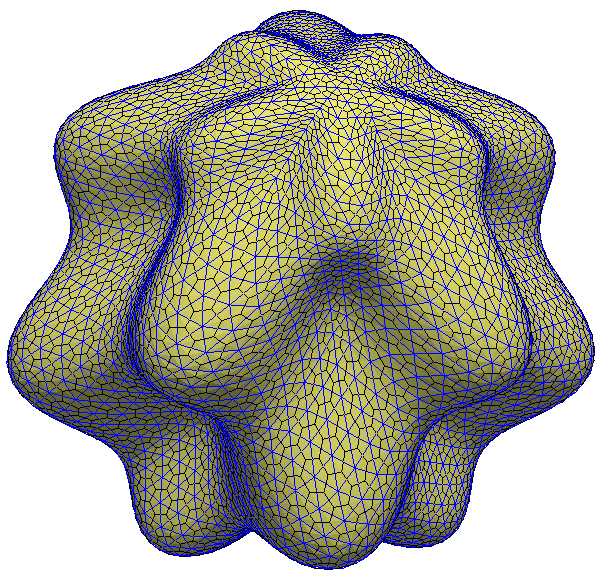
\includegraphics[width=0.35\linewidth]{bumpy_noRed_level5_tstep0_FT.png}
	\hspace{0.1\linewidth}
	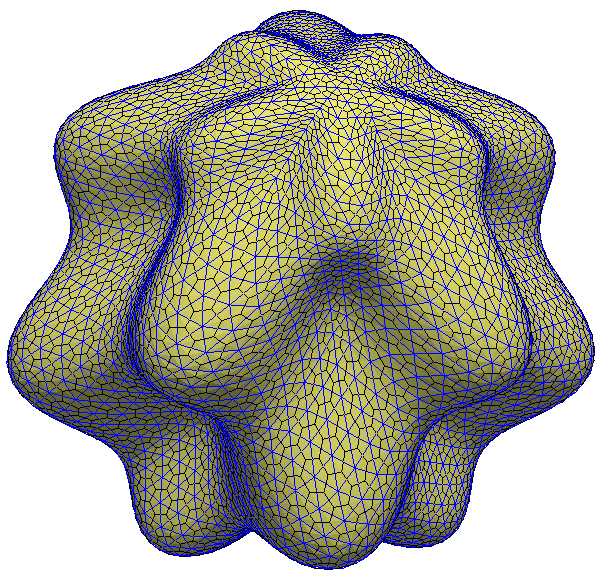
\includegraphics[width=0.35\linewidth]{bumpy_noRed_level5_tstep0_FT.png}
	\newline
	\includegraphics[width=0.35\linewidth]{bumpy_noRed_level5_tstep20.png}
	\hspace{0.1\linewidth}
	\includegraphics[width=0.35\linewidth]{bumpy_omega100_level5_tstep20.png}
	\newline
	\includegraphics[width=0.35\linewidth]{bumpy_noRed_level5_tstep50.png}
	\hspace{0.1\linewidth}
	\includegraphics[width=0.35\linewidth]{bumpy_omega100_level5_tstep50.png}
	\newline
	\includegraphics[width=0.35\linewidth]{bumpy_noRed_level5_tstep128.png}
	\hspace{0.1\linewidth}
	\includegraphics[width=0.35\linewidth]{bumpy_omega100_level5_tstep128.png}
	\newline
	%	\vspace{-5pt}
	\caption{Príklady obrázkov z ParaView.}\label{fig:bumpy_sphere} 
	%\vspace{-10pt}
\end{figure}

\begin{figure}[!h]
	\centering
	\vspace{-5pt}
	\begin{minipage}{.5\linewidth}
		\centering
		\includegraphics[width=0.95\linewidth]{vzduchovod1}
		\vspace{-5pt}
		\caption{Obrázok z ANSYS-u.}
		\label{fig:vzduchovod_geom}
	\end{minipage}%
	\begin{minipage}{.5\linewidth}
		\centering
		\includegraphics[width=0.95\linewidth]{vzduchovod2}
		\vspace{-5pt}
		\caption{Obrázok z ANSYS-u.}
		\label{fig:vzduchovod_mesh}
	\end{minipage}
	\vspace{-5pt}
\end{figure}

Pomocou balíka \verb|subcaption| sa dajú obrázky vložiť vedľa seba tak, ako vidíme na Obrázku~\ref{fig:matlab}, pričom môžu mať jeden hlavný popis a ďalšie podpopisy \ref{fig:matlab_2D}~resp.~\ref{fig:matlab_3D}.
\begin{figure}[!h]
	\centering
	\begin{subfigure}[b]{0.45\linewidth}
		\includegraphics[width=\linewidth]{matlab_2D}
		\caption{Graf funkcie jednej premennej (2D).}
		\label{fig:matlab_2D}
	\end{subfigure}
	\qquad
	\begin{subfigure}[b]{0.45\linewidth}
		\includegraphics[width=\linewidth]{matlab_3D}
		\caption{Graf funkcie v dvoch premenných (3D).}
		\label{fig:matlab_3D}
	\end{subfigure}
	\caption{Príklady obrázkov z MATLAB-u.}\label{fig:matlab}
\end{figure}


\subsection{Vytváranie obrázkov}

Z časti \ref{sec:vkladanie_obrazkov} už máme predstavu, ako vkladať existujúce obrázky (resp. výstupné obrázky zo softvéru, napríklad z ANSYS-u). V akom programe ale vytvárať nové grafy a obrázky? Toto je (prekvapujúco?) ťažká otázka.

\paragraph{Aké formáty používať?}

\begin{itemize}
	\item \textbf{Vektorová grafika:} PDF, EPS (LaTeX ale aj tak EPS skonvertuje na PDF).
	\item \textbf{Rastrová grafika:} PNG, JPG (odporúčam radšej PNG, lebo pri ukladaní do JPG resp. JPEG sa kvôli kompresii znižuje kvalita a vzniká šum).
\end{itemize}
Kvôli kvalite obrázkov \textbf{preferujte vektorovú grafiku} (ak je to možné a ak vektorový obrázok vyzerá dobre). V elektronickej verzii práce sú vektorové obrázky aj po priblížení stále pekné, hladké. Pri grafike, ktorá je tieňovaná (napr. plochy v 3D) je lepšie obrázok v dostatočnej kvalite uložiť ako raster. Vo všeobecnosti je dobré obrázky ukladať tak, aby boli orezané, bez veľkého nadbytočného orámovania okolo toho, čo nás zaujíma.


\paragraph{Mathematica.}

V softvéri Mathematica robiť viete, preto je dobrý nápad tvoriť grafy/obrázky v ňom. Pre export nepoužívajte screenshot, ale export:
\begin{itemize}
	\item \textbf{2D grafika:} \verb|pravý klik na obrázok/Save Graphic As/pdf|. Grafika bude automaticky vektorová.
	\item \textbf{3D grafika:} \verb|pravý klik na obrázok/Save Graphic As/png| (obrázok treba mať pred uložením dostatočne veľký). Je dobré ešte pred uložením obrázka odstrániť Bounding Box: \verb|pravý klik na| \verb|obrázok/| \verb|Trim| \verb|Bounding Box|, aby okolo obrázka nebolo zbytočne veľa bielej plochy.
\end{itemize}
Niekedy potrebujeme obrázok uložiť aj spolu s legendou (prípadne inými grafickými objektami), vtedy treba \verb|pravý klik na pravú lištu/Save Selection As/|, predtým je ešte vhodné vymazať \verb|Out[1]=| na ľavej strane. Obrázok sa dá uložiť aj pomocou príkazu \verb|Export| (zíde sa napríklad vtedy, keď potrebujete export automatizovať počas behu kódu alebo si ukladanie zautomatizovať).


\paragraph{MATLAB.}

Ak viete robiť MATLAB-e, prípadne v ňom programujete program k záverečnej práci, je dobrý nápad robiť grafy/obrázky v ňom. Pre export nepoužívajte screenshot, ale \verb|Save As| v okne Figure (aby sa ponuka \verb|Save As| zobrazila, treba podržať kurzor myši priamo nad obrázkom a kliknúť na prvú možnosť, pozri Obr.~\ref{fig:matlabfigures}) a vybrať formát (PDF resp. PNG). Ak z nejakého dôvodu potrebujete formát, ktorý nie je v ponuke (napr. EPS), sú aj ďalšie možnosti, napr. -- v okne Figure klik na \verb|File/Save As| a vybrať formát.\footnote{PDF tu nefunguje dobre, vloží obrázok do stredu A4.} Je praktické si obrázky ukladať aj vo formáte \verb|.fig|, aby ste ľahko mohli aj neskôr editovať rôzne nastavenia. Obrázok sa dá uložiť aj pomocou príkazu \verb|exportgraphics|, v ktorom si nastavíte aj formát. Viac informácii o ukladaní obrázkov nájdete na   \href{https://www.mathworks.com/help/matlab/creating_plots/save-figure-with-minimal-white-space.html}{stránke MathWorks}.
\begin{figure}[h!]
	\centering
	\includegraphics[width=0.7\linewidth]{figures/Matlab_figures}
	\caption{Uloženie obrázka v MATLAB-e.}
	\label{fig:matlabfigures}
\end{figure}



\paragraph{ParaView.}

Ak sú vaše dáta, resp. výsledky vhodné na vizualizáciu v ParaView, tak obrázky odtiaľ môžete ľahko exportovať. Platia podobné odporúčania, ako pri Mathematice a MATLAB-e. Ja tu pre všetky obrázky používam \verb|File/Save Screenshot/PNG| (alebo aj cez ikonu fotoaparátu na lište nad oknom \verb|RenderView|). V okne \verb|Save Screenshot Options| je potom vhodné nastaviť si v \verb|Coloring| pozadie na \verb|Transparent Background| alebo \verb|White| \verb|Bacground|. Pred exportom je vhodné vypnúť \verb|Show Orientation| \verb|Axes| a nastaviť okno tak, aby nebolo príliš veľa pozadia. 
Viac sa o exportovaní obrázkov píše \href{https://docs.paraview.org/en/v5.8/UsersGuide/savingResults.html}{tu na stránke ParaView}. V ParaView boli vytvorené Obrázky~\ref{fig:bumpy_sphere}.


\paragraph{Inkscape.}

\href{https://inkscape.org/}{Inkscape} je výborný program na vytváranie vektorovej grafiky. Zíde sa, keď potrebujete kresliť schematické obrázky (nie grafy funkcií). Pracuje s formátom SVG, ale môžete importovať/exportovať do mnohých formátov (aj PDF a EPS). Veľmi odporúčam doinštalovať \href{https://inkscape.org/~jcwinkler/%E2%98%85textext}{TexText extension}, aby ste do obrázkov mohli vpisovať LaTeX-ovské symboly a vzorce. Inkscape má \href{https://inkscape.org/learn/}{výborné tutorialy} (zrejme stačia Basic+Advanced), takže sa dá celkom rýchlo zvládnuť. V Inkscape bol vytvorený napríklad obrázok~\ref{fig:bod_v_rovine}. Keď už máte niečo nakreslené, export sa urobí takto:
\begin{enumerate}
	\item Označíte si, čo chcete exportovať.
	\item \verb|Ctrl+Shift+R| alebo \verb|Edit/Resize Page to Selection|.
	\item \verb|Ctrl+Shift+S| alebo \verb|File/Save As| a vybrať PDF. 
\end{enumerate}

\paragraph{Mathmeatica/Matlab/ParaView + Inkscape}

Ak do obrázka potrebujete doplniť popisky alebo vzorce, ktoré nedokážete dobre urobiť v Mathematice (resp. inom softvéri), často je praktickejšie na to použiť vhodný editor -- napríklad Inkscape. Takouto kombinovanou technikou (Mathematica+Inkscape) bol vytvorený Obrázok~\ref{fig:rezy} (po pribížení zistíte, čo bolo dorobené v Inkscape).
\begin{figure}[h]
	%\vspace{-10pt}
	\centering
	\includegraphics[width=0.8\linewidth]{fig_rezy}
	%\vspace{-10pt}
	\caption{Mathematica + dorobenie v Inkscape.} \label{fig:rezy}
	%	\vspace{-10pt}
\end{figure}


\paragraph{Programovanie obrázkov v LaTeX-u.}

Kvalitné obrázky sa dajú naprogramovať aj priamo v LaTeX-u. Nepoužívam to, ale sú ľudia, čo na tom frčia. Tu je niekoľko odkazov na túto možnosť:
\begin{itemize}
	\item \href{https://www.overleaf.com/learn/latex/TikZ_package}{Balík TikZ} je asi najlepší. \href{https://texample.net/tikz/examples/}{Na tejto stránke} nájdete veľké množstvo príkladov -- pre predstavu, čo všetko a ako sa dá nakresliť.
	\item \href{https://en.wikibooks.org/wiki/LaTeX/Picture}{Prostredie picture}, príkladom je Obrázok~\ref{fig:picture_test}.
	\item \href{https://en.wikipedia.org/wiki/PSTricks}{Balík PSTricks}
\end{itemize}
Z niektorých programov na kreslenie obrázkov sa dá TeX-ovský kód generujúci obrázok exportovať (napríklad Inkscape $\rightarrow$ PStricks).
\begin{figure}[!h]
	\centering
	\setlength{\unitlength}{0.8cm}
	\begin{picture}(6,5)
		\thicklines
		\put(1,0.5){\line(2,1){3}}
		\put(4,2){\line(-2,1){2}}
		\put(2,3){\line(-2,-5){1}}
		\put(0.7,0.3){$A$}
		\put(4.05,1.9){$B$}
		\put(1.7,2.95){$C$}
		\put(3.1,2.5){$a$}
		\put(1.3,1.7){$b$}
		\put(2.5,1.05){$c$}
		\put(0.3,4){$F=\sqrt{s(s-a)(s-b)(s-c)}$}
		\put(3.5,0.4){$\displaystyle s:=\frac{a+b+c}{2}$}
	\end{picture}
	\caption{Obrázok vytvorený pomocou prostredia picture.}
	\label{fig:picture_test}
\end{figure}


\section{Tabuľky}

Jednoduchá tabuľka bez popisu sa robí takto:

\begin{tabular}{|r|r|r|}
	\hline
	2 &   4 & 4.5 \\ \hline
	3 &   1 &   5 \\
	18 & 4.5 &   5 \\ \hline
\end{tabular}

Tabuľky v záverečnej práci by ale mali mať popis, tu je príklad s popisom: 
\begin{table}[!h]
	\centering
	\caption{The $L^2$ EOC for the case with no redistribution.}
	\begin{tabular}{rlrrr}
		\hline
		$n_V$ & $\tau$     & $N$ & $ L^2\mbox{ error}$ &  EOC \\ \hline
		122 & 0.04       &   2 &            1.43e-02 &      \\
		482 & 0.01       &   8 &            3.35e-03 & 2.10 \\
		1922 & 0.0025     &  32 &            8.07e-04 & 2.05 \\
		7682 & 0.000625   & 128 &            1.95e-04 & 2.05 \\
		30722 & 0.00015625 & 512 &            4.64e-05 & 2.07 \\ \hline
	\end{tabular}
	\label{tab:resultsDDFV}
\end{table}

Ešte jeden príklad s použitím farby a definovaním šírky stĺpcov je v Tabuľke~\ref{tab:Veliciny}. Viac o tabuľkách nájdete aj s peknými príkladmi a zdrojovými kódmi \href{https://en.wikibooks.org/wiki/LaTeX/Tables#Basic_examples}{napríklad tu na wikibooks}.
\begin{table}[h]
	\centering
	\caption{Prehľad veličín.} \label{tab:Veliciny}
	\begin{tabular}{|l|l|p{45mm}|p{60mm}|}
		\hline
		\rowcolor[gray]{.8}
		Veličina & Jednotka & Názov & Popis  \\ \hline
		$u(x,t)$ & $\si{K}$ & Teplota v~mieste $x$ a čase $t$ &   \\ \hline
		$c(x)$ & $\si{J/kg.K}$ & Merná tepelná kapacita & Množstvo tepla (J) potrebné na zohriatie 1 kg látky o 1 K  \\ \hline
		$\rho(x)$ & $\si{kg/m^3}$ & Hustota &  \\ \hline
		$f(x,t)$ & $\si{J/m^3}$s & Intenzita (hustota) \newline zdrojov tepla & Množstvo tepla (J) vyprodukované v~$\SI{1}{m^3}$ za 1 s   \\ \hline
		$q(x,t)$ & $\si{J/m^2.s}$ & Hustota tepelného toku & Množstvo tepla, ktoré prejde prierezom $\SI{1}{m^2}$ za 1 s  \\ \hline
	\end{tabular}
\end{table}

\paragraph{Dôležitý tip.}
Vytvárať tabuľku priamo v zdrojovom kóde v LaTeX editore môže byť pri väčších tabuľkách dosť neprehľadné a neefektívne, odporúčam \href{https://www.tablesgenerator.com/}{tento výborný online nástroj}. Môžete tam ľahko vytvoriť novú tabuľku, vložiť (copy-paste) existujúcu tabuľku (napríklad z Excelu), či importovať z .csv, následne efektívne upravovať (perpisovať, meniť orámovanie, merge-ovať bunky, meniť farby,...), a nakoniec jedným klikom vygenerovať zodpovedajúci kód pre TeX-ovskú tabuľku, ktorý si vložíte do práce.

\section{Vkladanie pseudokódu a kódu}

V záverečných prácach na MPM je niekedy vhodné vysvetliť váš algoritmus alebo kód. Na písanie pseudokódov existuje veľa balíkov, prehľad nájdete \href{https://www.overleaf.com/learn/latex/Algorithms}{na stránke Overleaf-u} alebo \href{https://en.wikibooks.org/wiki/LaTeX/Algorithms#The_algorithm_environment}{na wikibooks}. Algoritmus~\ref{alg:algorithm2e_exmp} je príkladom použitia balíka \verb|algorithm2e|.

\RestyleAlgo{ruled}
\begin{algorithm}[!h]
	\caption{An algorithm with caption}\label{alg:algorithm2e_exmp}
	\KwData{$n \geq 0$}
	\KwResult{$y = x^n$}
	$y \gets 1$\;
	$X \gets x$\;
	$N \gets n$\;
	\While{$N \neq 0$}{
		\eIf{$N$ is even}{
			$X \gets X \times X$\;
			$N \gets \frac{N}{2} $
		}{\If{$N$ is odd}{
				$y \gets y \times X$\;
				$N \gets N - 1$\;
			}
		}
	}
\end{algorithm}

Ak potrebujete do práce vložiť nejakú časť kódu, vodný je napríklad balík \verb|listings|. Jednoduché použitie je tu:
\begin{lstlisting}
	#include <stdio.h>
	int main() {
		// printf() displays the string inside quotation
		printf("Hello, World!");
		return 0;
	}
\end{lstlisting}

Dá sa pohrať s formátovaním, nastaviť si farby, font a podobne. Nastavenie som vložil sem do kódu. Ak budete nejaké používať, dajte si ho do preambuly. Viac o vkladaní kódu sa dočítate v dokumentácii balíka \verb|listings|.

% nastavenie farieb
\definecolor{dkgreen}{rgb}{0,0.6,0}
\definecolor{gray}{rgb}{0.5,0.5,0.5}
\definecolor{mauve}{rgb}{0.58,0,0.82}

% nastavenie balika listings
\lstset{frame=tb,
	language=C,
	aboveskip=3mm,
	belowskip=3mm,
	showstringspaces=false,
	columns=flexible,
	basicstyle={\small\ttfamily},
	numbers=none,
	numberstyle=\tiny\color{gray},
	keywordstyle=\color{blue},
	commentstyle=\color{dkgreen},
	stringstyle=\color{mauve},
	breaklines=true,
	breakatwhitespace=true,
	tabsize=3
}

\begin{lstlisting}
	#include <stdio.h>
	int main() {
		// printf() displays the string inside quotation
		printf("Hello, World!");
		return 0;
	}
\end{lstlisting}

	\chapter{Záver}

V závere zhrniete, čomu sa venovala vaša práca, ako sa vám podarilo naplniť stanovené ciele a k akým výsledkom ste prišli. Môžete zhodnotiť váš postup riešenia problému, jeho výhody/nevýhody. V závere je vhodné aj naznačiť, akými smermi by sa dalo v práci pokračovať, aké zostali nevyriešené otázky, kde vidíte možnosti vylepšenia a podobne.


	% ====== Bibliografia a prilohy ======
	\nocite{*} % Vypise v bibliografii aj zroje, ktore neboli citovane
	\printbibliography[heading=bibintoc]
	
	\chapter*{Použitie umelej inteligencie}
\addcontentsline{toc}{chapter}{Použitie umelej inteligencie}

Od 1.12.2024 je v platnosti predpis \uv{Používanie umelej inteligencie na STU
v Bratislave}, nájdete ho aj v priečinku \verb|ZaverecnaPracaMPM\dokumenty|. Predpis sa týka aj záverečných prác. Ak ste použili AI, treba to v práci na tomto mieste deklarovať a uviesť podrobnosti. Niekoľko príkladov (uvedených v predpise) je tu:

\begin{itemize}
	\item \textit{OpenAI (2024), ChatGPT, časť 2.1, generovanie textu}
	
	\item \textit{OpenAI (2024), ChatGPT, časť 5.4, generovanie kódu na vizualizáciu výsledkov, jazyk Pyton}
	
	\item \textit{Google, Geminy (2024), získanie experimentálnych dát pre experiment v časti 7.2.3}
	
	\item \textit{DeepL (2024), https://www.deepl.com/en/translator, preklady viacerých častí textu}
	
	\item \textit{Grammarly, https://app.grammarly.com, gramatická korekcia celého textu}
\end{itemize}
	
	
	%\includepdf[pages=-,pagecommand={}]{documents/priloha1.pdf} % pripadne prilohy
\end{document}